% 使用 XeLaTeX + ctex + graphicx；假定本文文件位于项目根目录。

\begin{figure}[htbp]
\centering
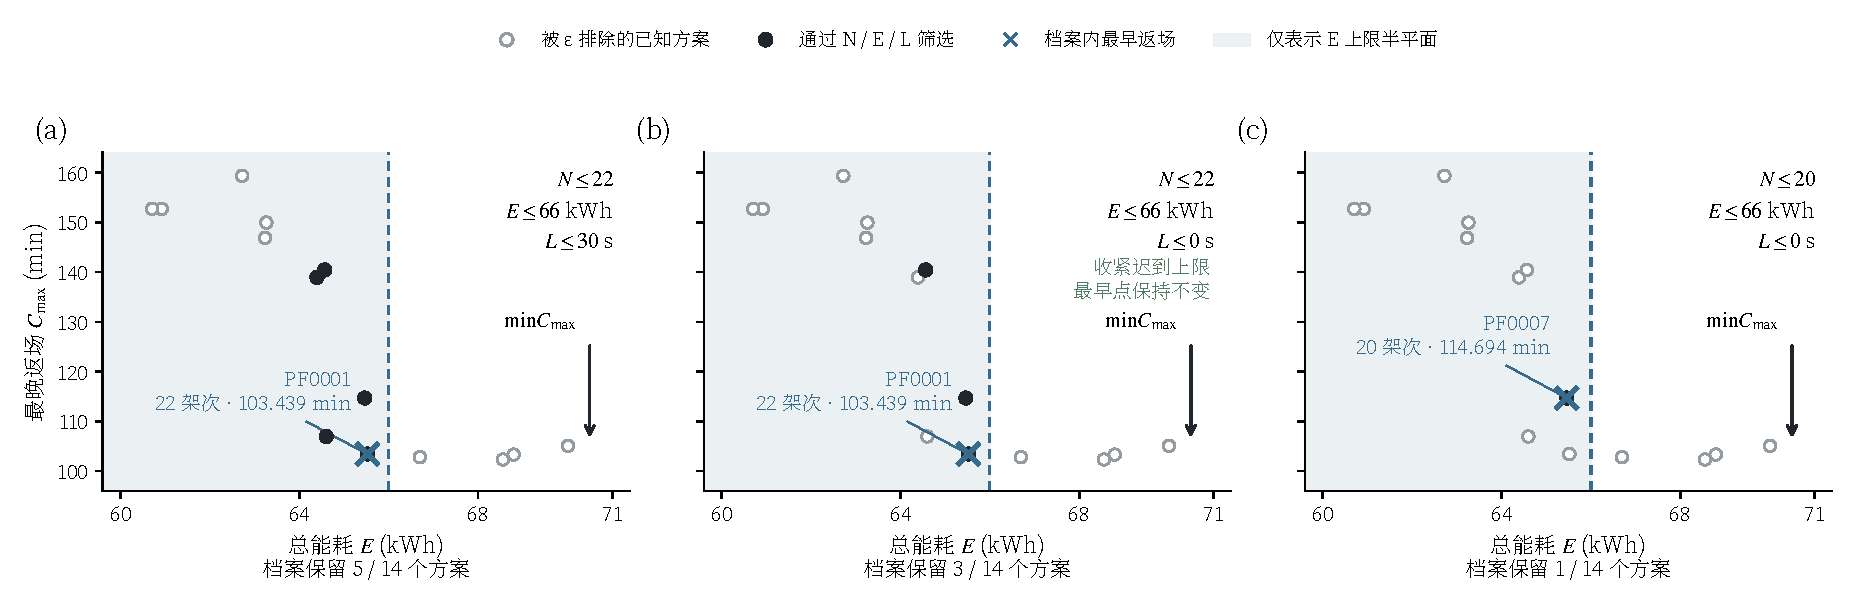
\includegraphics[width=\textwidth]{问题二/机理图/图1_epsilon约束与四目标条件筛选.pdf}
\caption{最终档案中14个已核验方案的能耗—最晚返场时间投影。迟到上限由30 s收紧至0 s时，符合条件的方案由5个减少至3个，档案内最早返场方案保持不变；进一步将架次上限收紧为20后，仅余1个方案。蓝色背景仅表示能耗上限，标记同时考虑架次和迟到条件。结果为有限档案筛选，不构成ε子问题全局最优认证。}
\label{fig:q2-mechanism-1}
\end{figure}

\begin{figure}[htbp]
\centering
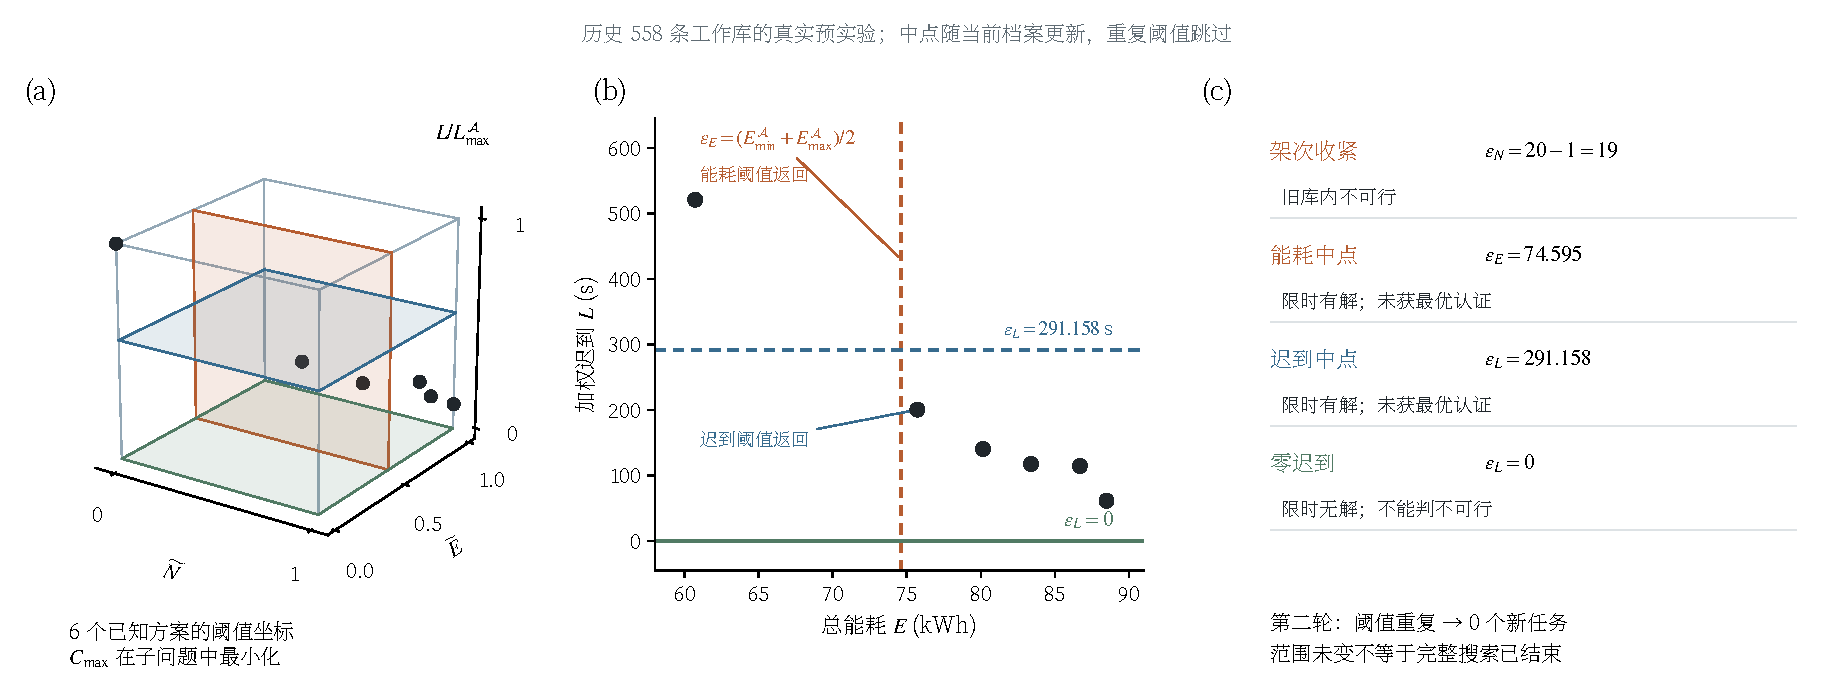
\includegraphics[width=\textwidth]{问题二/机理图/图2_自适应epsilon阈值与真实求解状态.pdf}
\caption{旧558条候选工作库上的自适应ε阈值构造与实际求解状态。档案范围生成架次减一、能耗中点、迟到中点及零迟到四种试探；对应状态来自各自任务日志。第二轮阈值重复而跳过，本次有限试探不代表完整目标空间枚举。}
\label{fig:q2-mechanism-2}
\end{figure}

\begin{figure}[htbp]
\centering
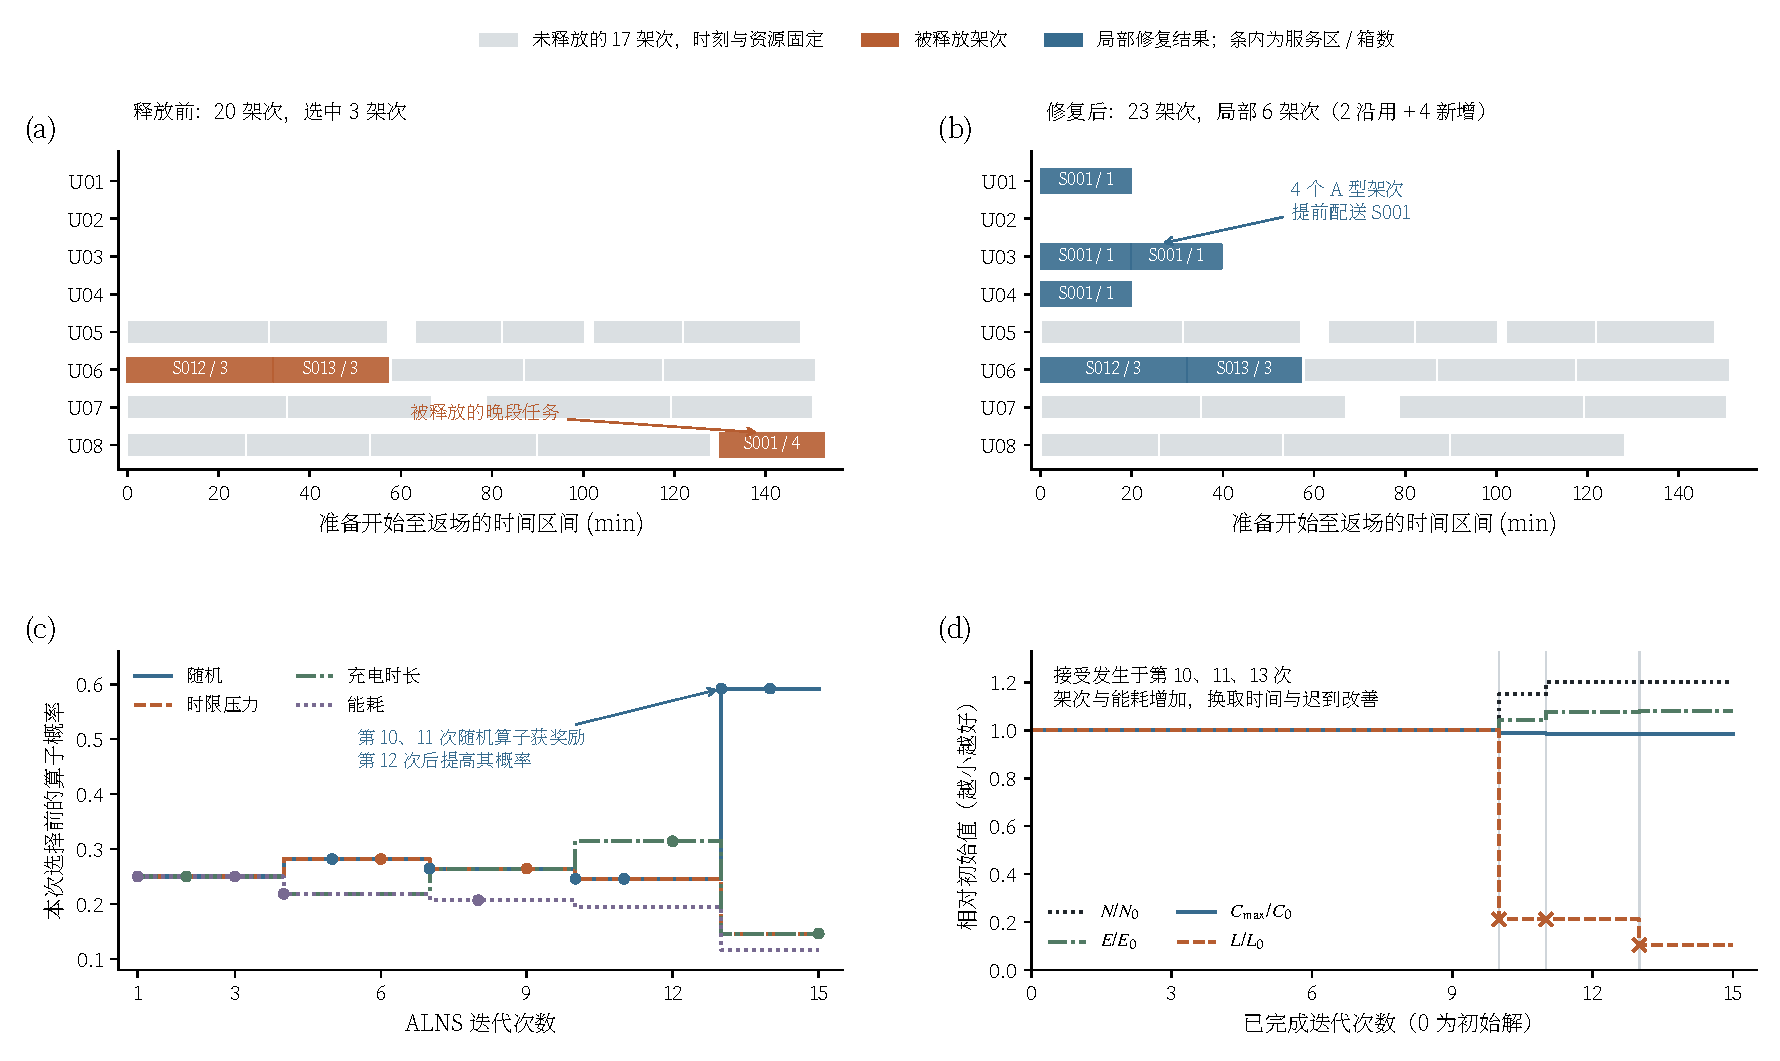
\includegraphics[width=\textwidth]{问题二/机理图/图3_ALNS破坏修复与自适应算子.pdf}
\caption{旧候选库上一次15步ALNS运行及第10次局部修复。释放3架次后，局部解包含2条沿用路线和4条新增路线；其余17架次的资源与时刻固定。下排显示本次选择前的算子概率和按接受事件重建的当前解目标轨迹。架次与能耗增加，同时完成时间和迟到降低。}
\label{fig:q2-mechanism-3}
\end{figure}

\begin{figure}[htbp]
\centering
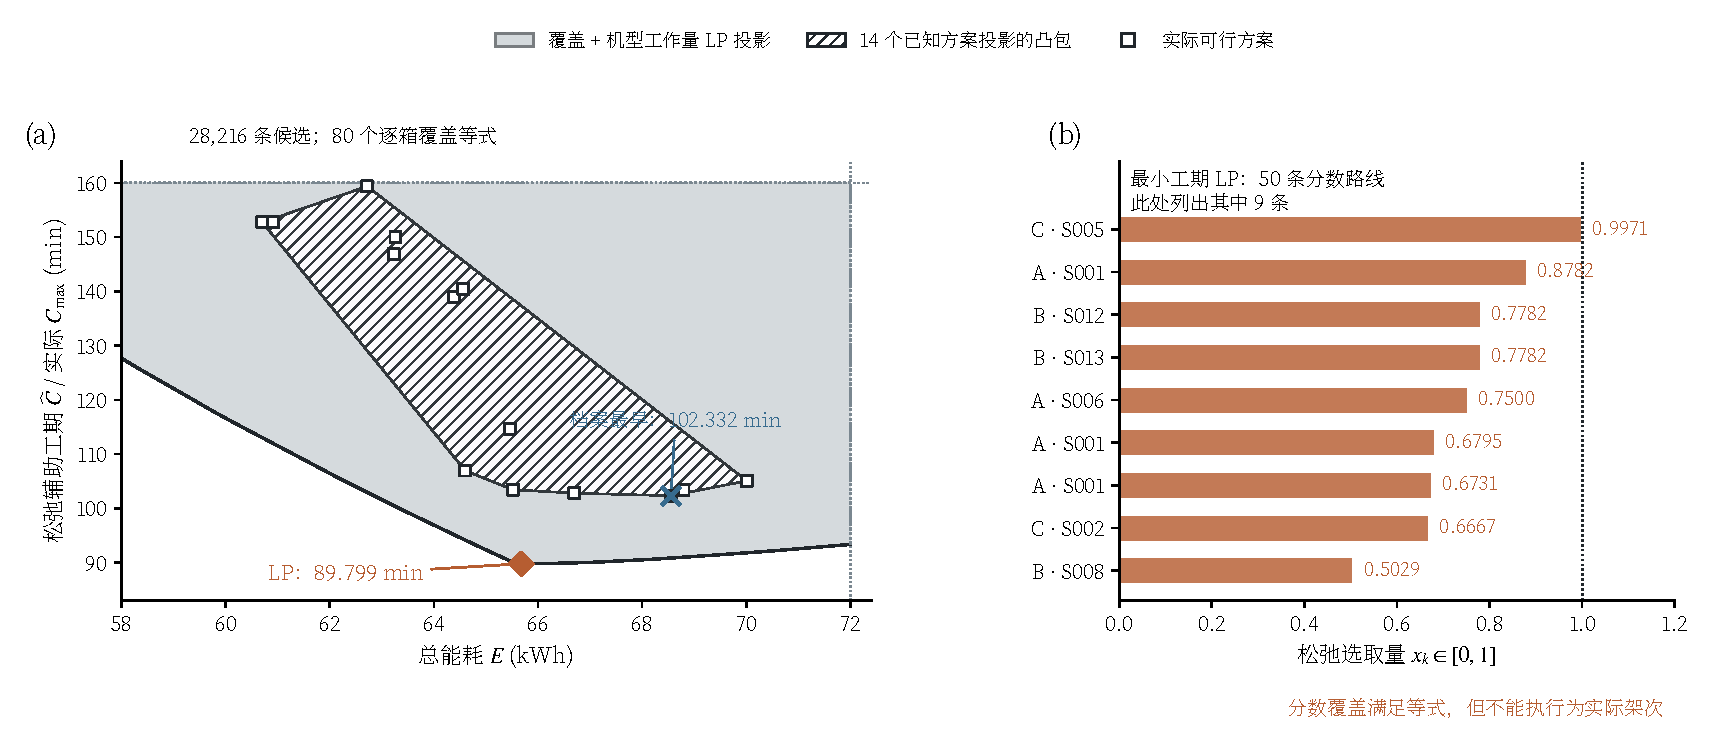
\includegraphics[width=\textwidth]{问题二/机理图/图4_覆盖工作量松弛域与分数解.pdf}
\caption{最终28216条候选库的覆盖—机型工作量松弛在能耗与辅助工期显示窗内的投影，以及14个已知可行方案投影的凸包。边界通过原LP支持函数逐边数值核验；点状线表示人工显示窗边界。斜线凸包内部和右图中的分数路线均不代表可执行调度。该下界仅适用于相同候选库和物理假设。}
\label{fig:q2-mechanism-4}
\end{figure}

\begin{figure}[htbp]
\centering
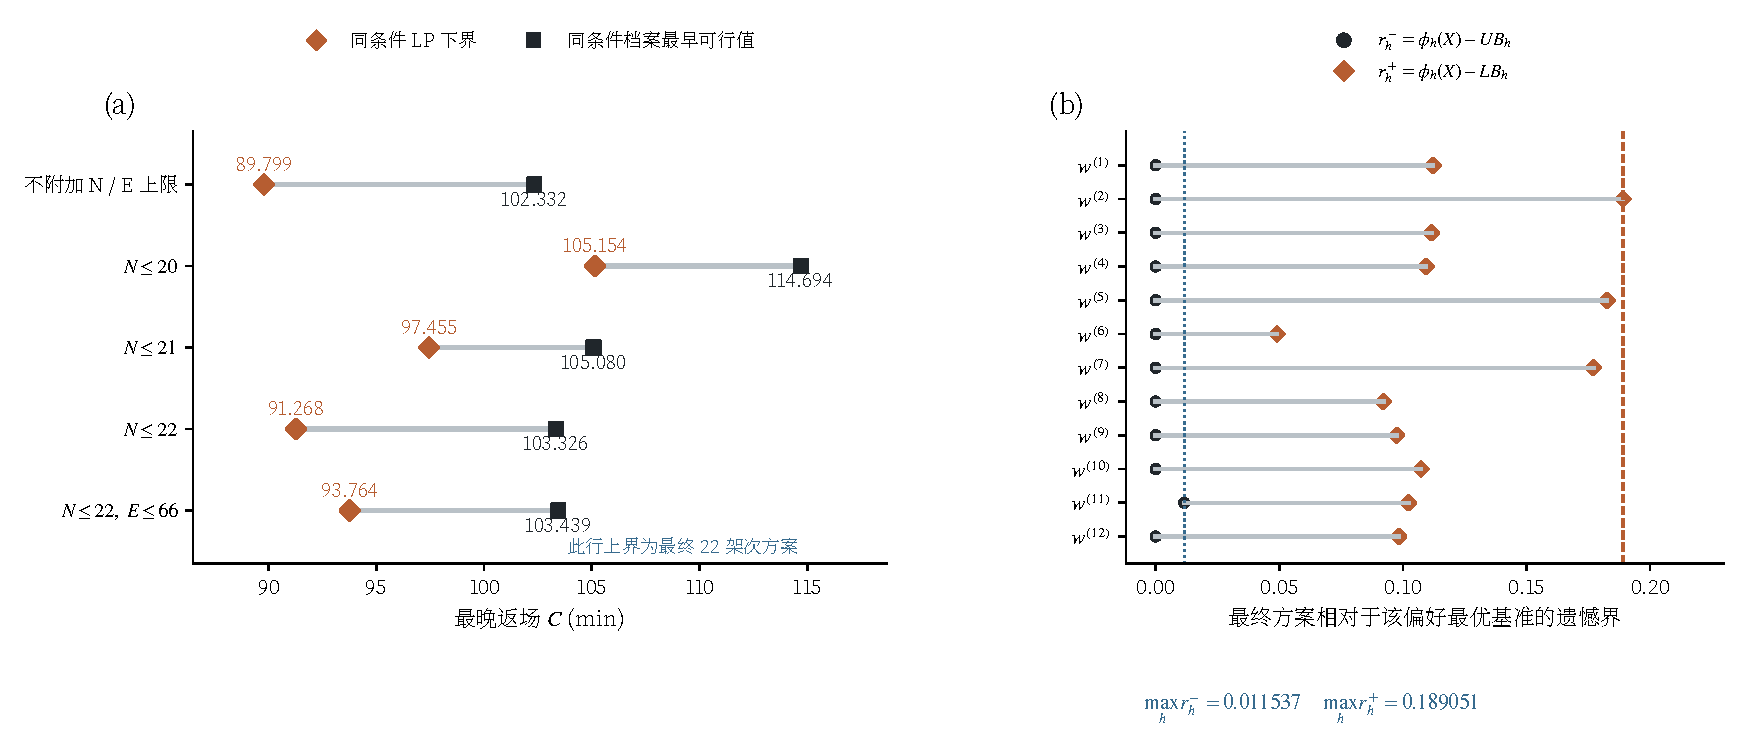
\includegraphics[width=\textwidth]{问题二/机理图/图5_同条件下界与最坏遗憾区间.pdf}
\caption{相同最终候选库下五种约束情景的时间松弛下界与对应档案最早可行上界，以及最终方案在12个冻结偏好极点上的遗憾上下界。所有比较保持候选库、评价尺度和情景条件一致。区间表示松弛下界至已知可行上界的差距，不提供完整原问题全局最优认证。}
\label{fig:q2-mechanism-5}
\end{figure}
